\documentclass[tikz]{standalone}

\usetikzlibrary{fit,positioning}
\pgfdeclarelayer{z1}
\pgfdeclarelayer{z2}
\pgfdeclarelayer{z3}
\pgfdeclarelayer{z4}
\pgfsetlayers{main,z1,z2,z3,z4}

\begin{document}
	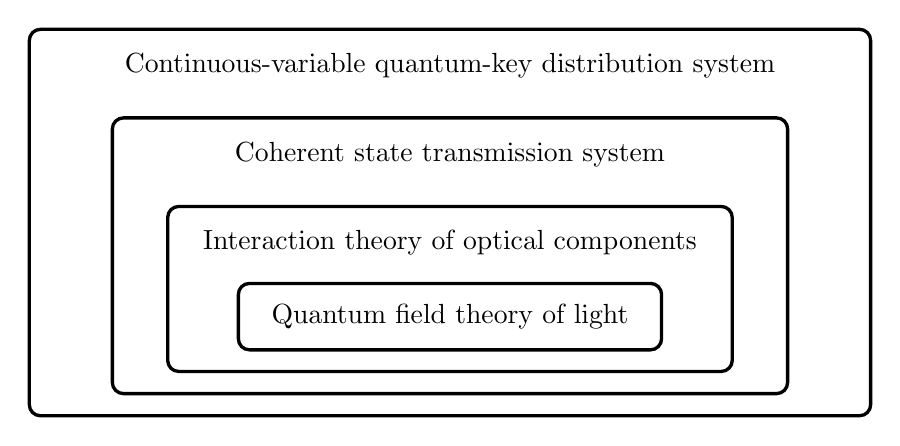
\begin{tikzpicture}[
		box/.style={draw, very thick, rectangle, rounded corners, fill=white, align=center, inner xsep=12pt, inner ysep=4pt},
	]
		\begin{pgfonlayer}{z4}
			\node[box, minimum height=24pt] (A) {Quantum field theory of light};
		\end{pgfonlayer}
		\begin{pgfonlayer}{z3}
			\node[box, fit=(A), yshift=10pt, text depth=40pt, text width=180] (B) {Interaction theory of optical components};
		\end{pgfonlayer}
		\begin{pgfonlayer}{z2}
			\node[box, fit=(A), yshift=22pt, text depth=80pt, text width=220pt] {Coherent state transmission system};
		\end{pgfonlayer}
		\begin{pgfonlayer}{z1}
			\node[box, fit=(A), yshift=34pt, text width=280pt, text depth=120pt] {Continuous-variable quantum-key distribution system};
		\end{pgfonlayer}
	\end{tikzpicture}
\end{document}
